\section{Approach Adopted}

edw

to keimeno

pou tha leei

panw katw

ti ginetai

s'auto to kefalaio

DHLADH THA ESTIAZEI STO WS 'H LDAP

\newpage


\section{Design Methods}
\subsection{Recommendations and standards}
\subsubsection{Grid Monitoring Architecture}
\nomenclature{GMA}{Grid Monitoring Architecture}
%% TODO producer-consumer plot
\newpage

\subsubsection{R-GMA}
%% TODO R-GMA literature
The rgma client is no longer configured in SL5
\nomenclature{R-GMA}{Relational Grid Monitoring Architecture}


\newpage
\subsubsection{GLUE Schema}
gained wide acceptance given its adoption by Globus MDS3


GLUE schema came to provide the interoperability needed between US and European Physics Grid Projects. As a standard, a common schema was introduced to describe and monitor the grid resources. Major components include:
\begin{enumerate}
\item Computing Element (CE)
\item Storage Element (SE)
\item Network Element (NE)
\end{enumerate}

The implementation of Glue schema may be using LDAP, XML or SQL. The MDS implementation of the Glue schema in this project includes the core Information Provider and the Ganglia Interface for the cluster information.
\nomenclature{GLUE}{Grid Laboratory Uniform Environment}
\newpage

\begin{figure}[htb]
\centering
 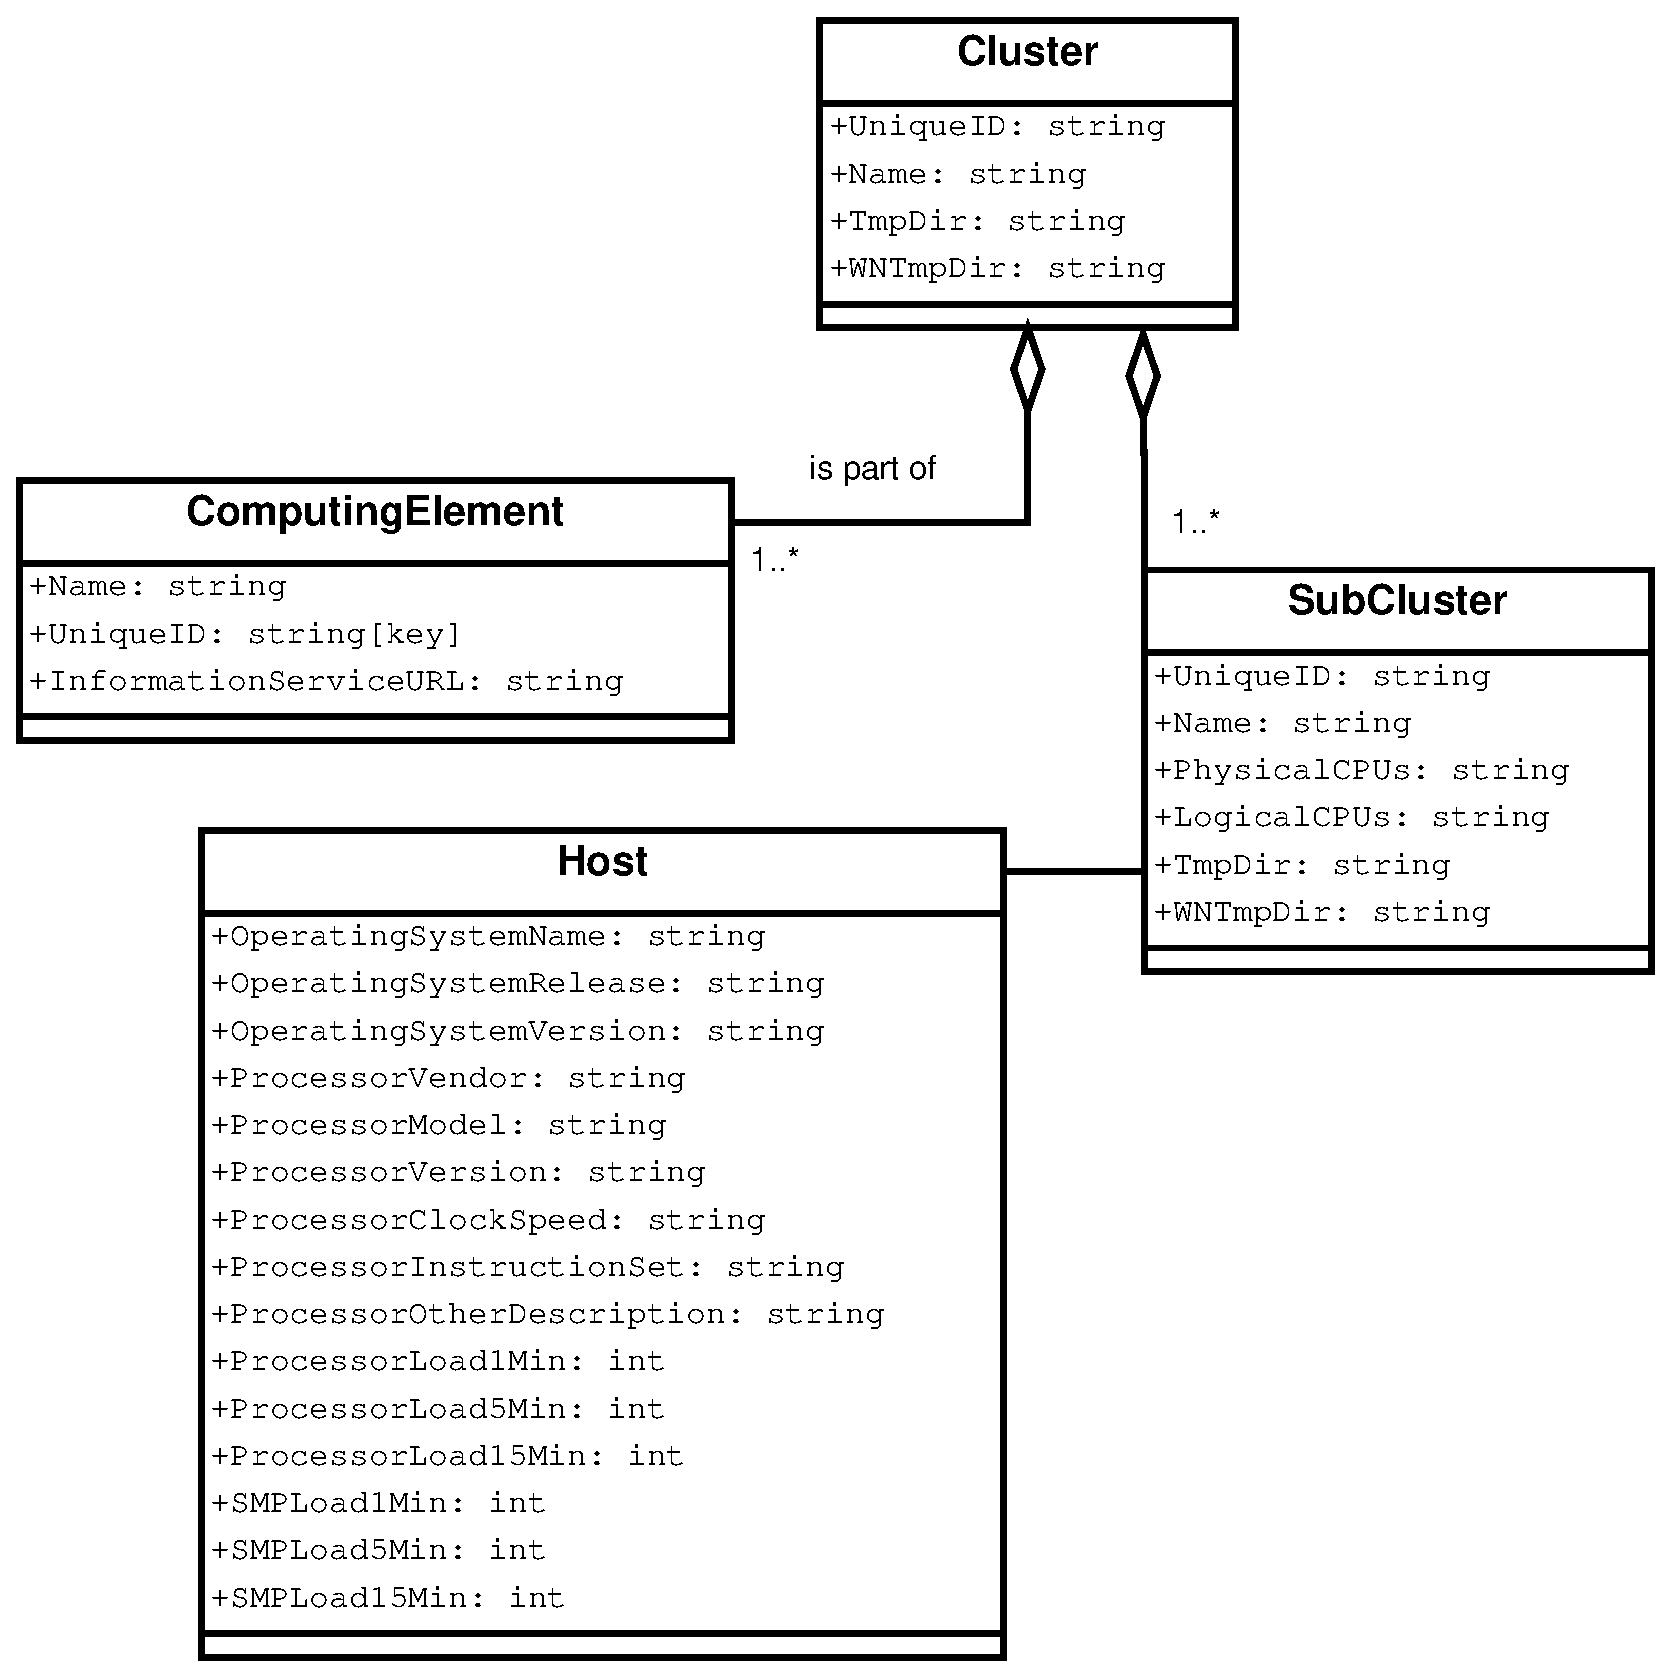
\includegraphics[width=5in]{images/gluece_ext.eps}
\caption{GLUE schema 2.0 extention for Host and SMP Load}
\label{figure:gluece_ext}
\end{figure}

\newpage

\subsection{Information Infrastructure}
% TODO to MDS me dika mou logia
To design the Information Infrastructure for distributed computing applications some requirements have been considered such as performance, scalability, cost and uniformity.

Because grid computing applications usually operate in large scale installations, there are performance requirements for the information infrastructure. It should allow rapid access to configuration information that is frequently used, using {\bf caching to query periodically each host or index server for the metrics}.

The number of components in a grid infrastructure scales up to hundreds of thousands of nodes, and these components should be available for queries by many different tools. That information should be discoverable using information indexes.

Deployments, maintenance and operations in a large installation of many systems has operational costs for human resources. The information system should automaticaly discover and serve the availability paths for applications and grid resources/servives.

Because of the large number of different heterogeneous networks of nodes and clusters, there is a need of uniformity. Uniformity helps to simplify the developers to build applications that give better configuration decisions. APIs for common operations and data models for the representation of that information. Resources are devided in groups of computing, storage, network elements, etc.

The solution proposed by GLUE standard and X.500 (Directory Service) is the key feature to scale, and get uniformity. It may be used to provide extensible distributed directory services. It is optimised for reads, its binary-tree like hierarchy and usually backend data structure provides a framework that well organize the information that need to be delivered by an Information Infrastructure.\cite{mds1}

\section{Data-acquisition Systems}
plugins that take metrics (SAM) and send results to nagios:

https://tomtools.cern.ch/confluence/display/SAMDOC/Grid+probes

http://nationalgridservice.blogspot.com/2010/10/nagios-myegee-and-myegi.html

4 layers to performance investigation:
\begin{enumerate}
  \item Storage elements
  \item Sites
  \item VOs
  \item Middleware
\end{enumerate}
3 benchmarking categories
\begin{enumerate}
  \item micro-benchmarks
  \item micro-kernels
  \item application kernels
\end{enumerate}
Benchmarking

HPL
\cite{gridbench}

CE performance
free processors
MFLOPS
MIPS (instructions per second)
free RAM

SE performance
IOPS
free space

EGI accounting portal: CPU usage metrics aggregated for accounting.
\newpage

\subsection{Metrics}\label{subsec:metrics}

{\bf CPU load} is taken using the pseudo /proc/loadavg file which in turn is
filled by Linux kernel's CALC\_LOAD macro. This function takes 3 parameters.
The load-average bucket, a $y$ constant that is calculated using formula
\[
y=\frac{2^{11}}{2^{((5log_2(e))/60x)}}
\]
for values $x=1$, $x=5$ and $x=15$ (where x represent the minutes and y the
exponent constant), and the number of how many processes are in the queue, in
running or uninterruptible state.

\begin{figure}[htb]
\centering
 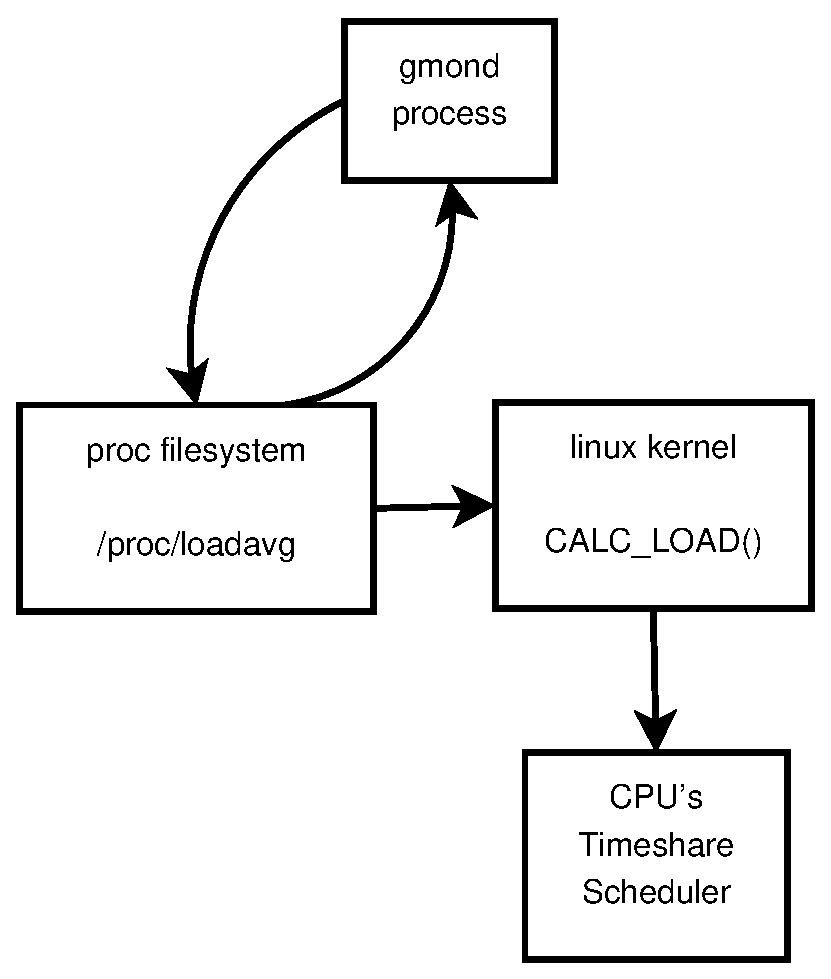
\includegraphics[width=3in]{images/calc_load.eps}
\caption{Load Average calculation}
\label{figure:calc_load}
\end{figure}

\newpage

\subsection{Ganglia}

The metrics about load in one, five and fifteen minutes are taken from Gmond daemon through the proc filesystem as seen in Figure \ref{figure:calc_load}. These values are multicasted using a UDP message on the network, only if the value has been changed from the previous one taken. There is also a time thresohold that after that time the value is been sent again, even if it haven't changed, so new hosts on the network may gather the data needed for their Gmond. Each host of a cluster have the information about the metrics of itself and each other node, so it stores the whole cluster state. Using loopback interface, every Gmond sends its metrics to itself.

If a TCP connection on the Gmond listening port 8649 is made, Gmond writes a full cluster state of metrics in XML including its DTD. There is a typical access list in the configuration called trusted hosts, and of course every node that is in the cluster that a specific node is configured to be part of, is allowed to connect to get the XML.

\begin{figure}[htb]
\centering
 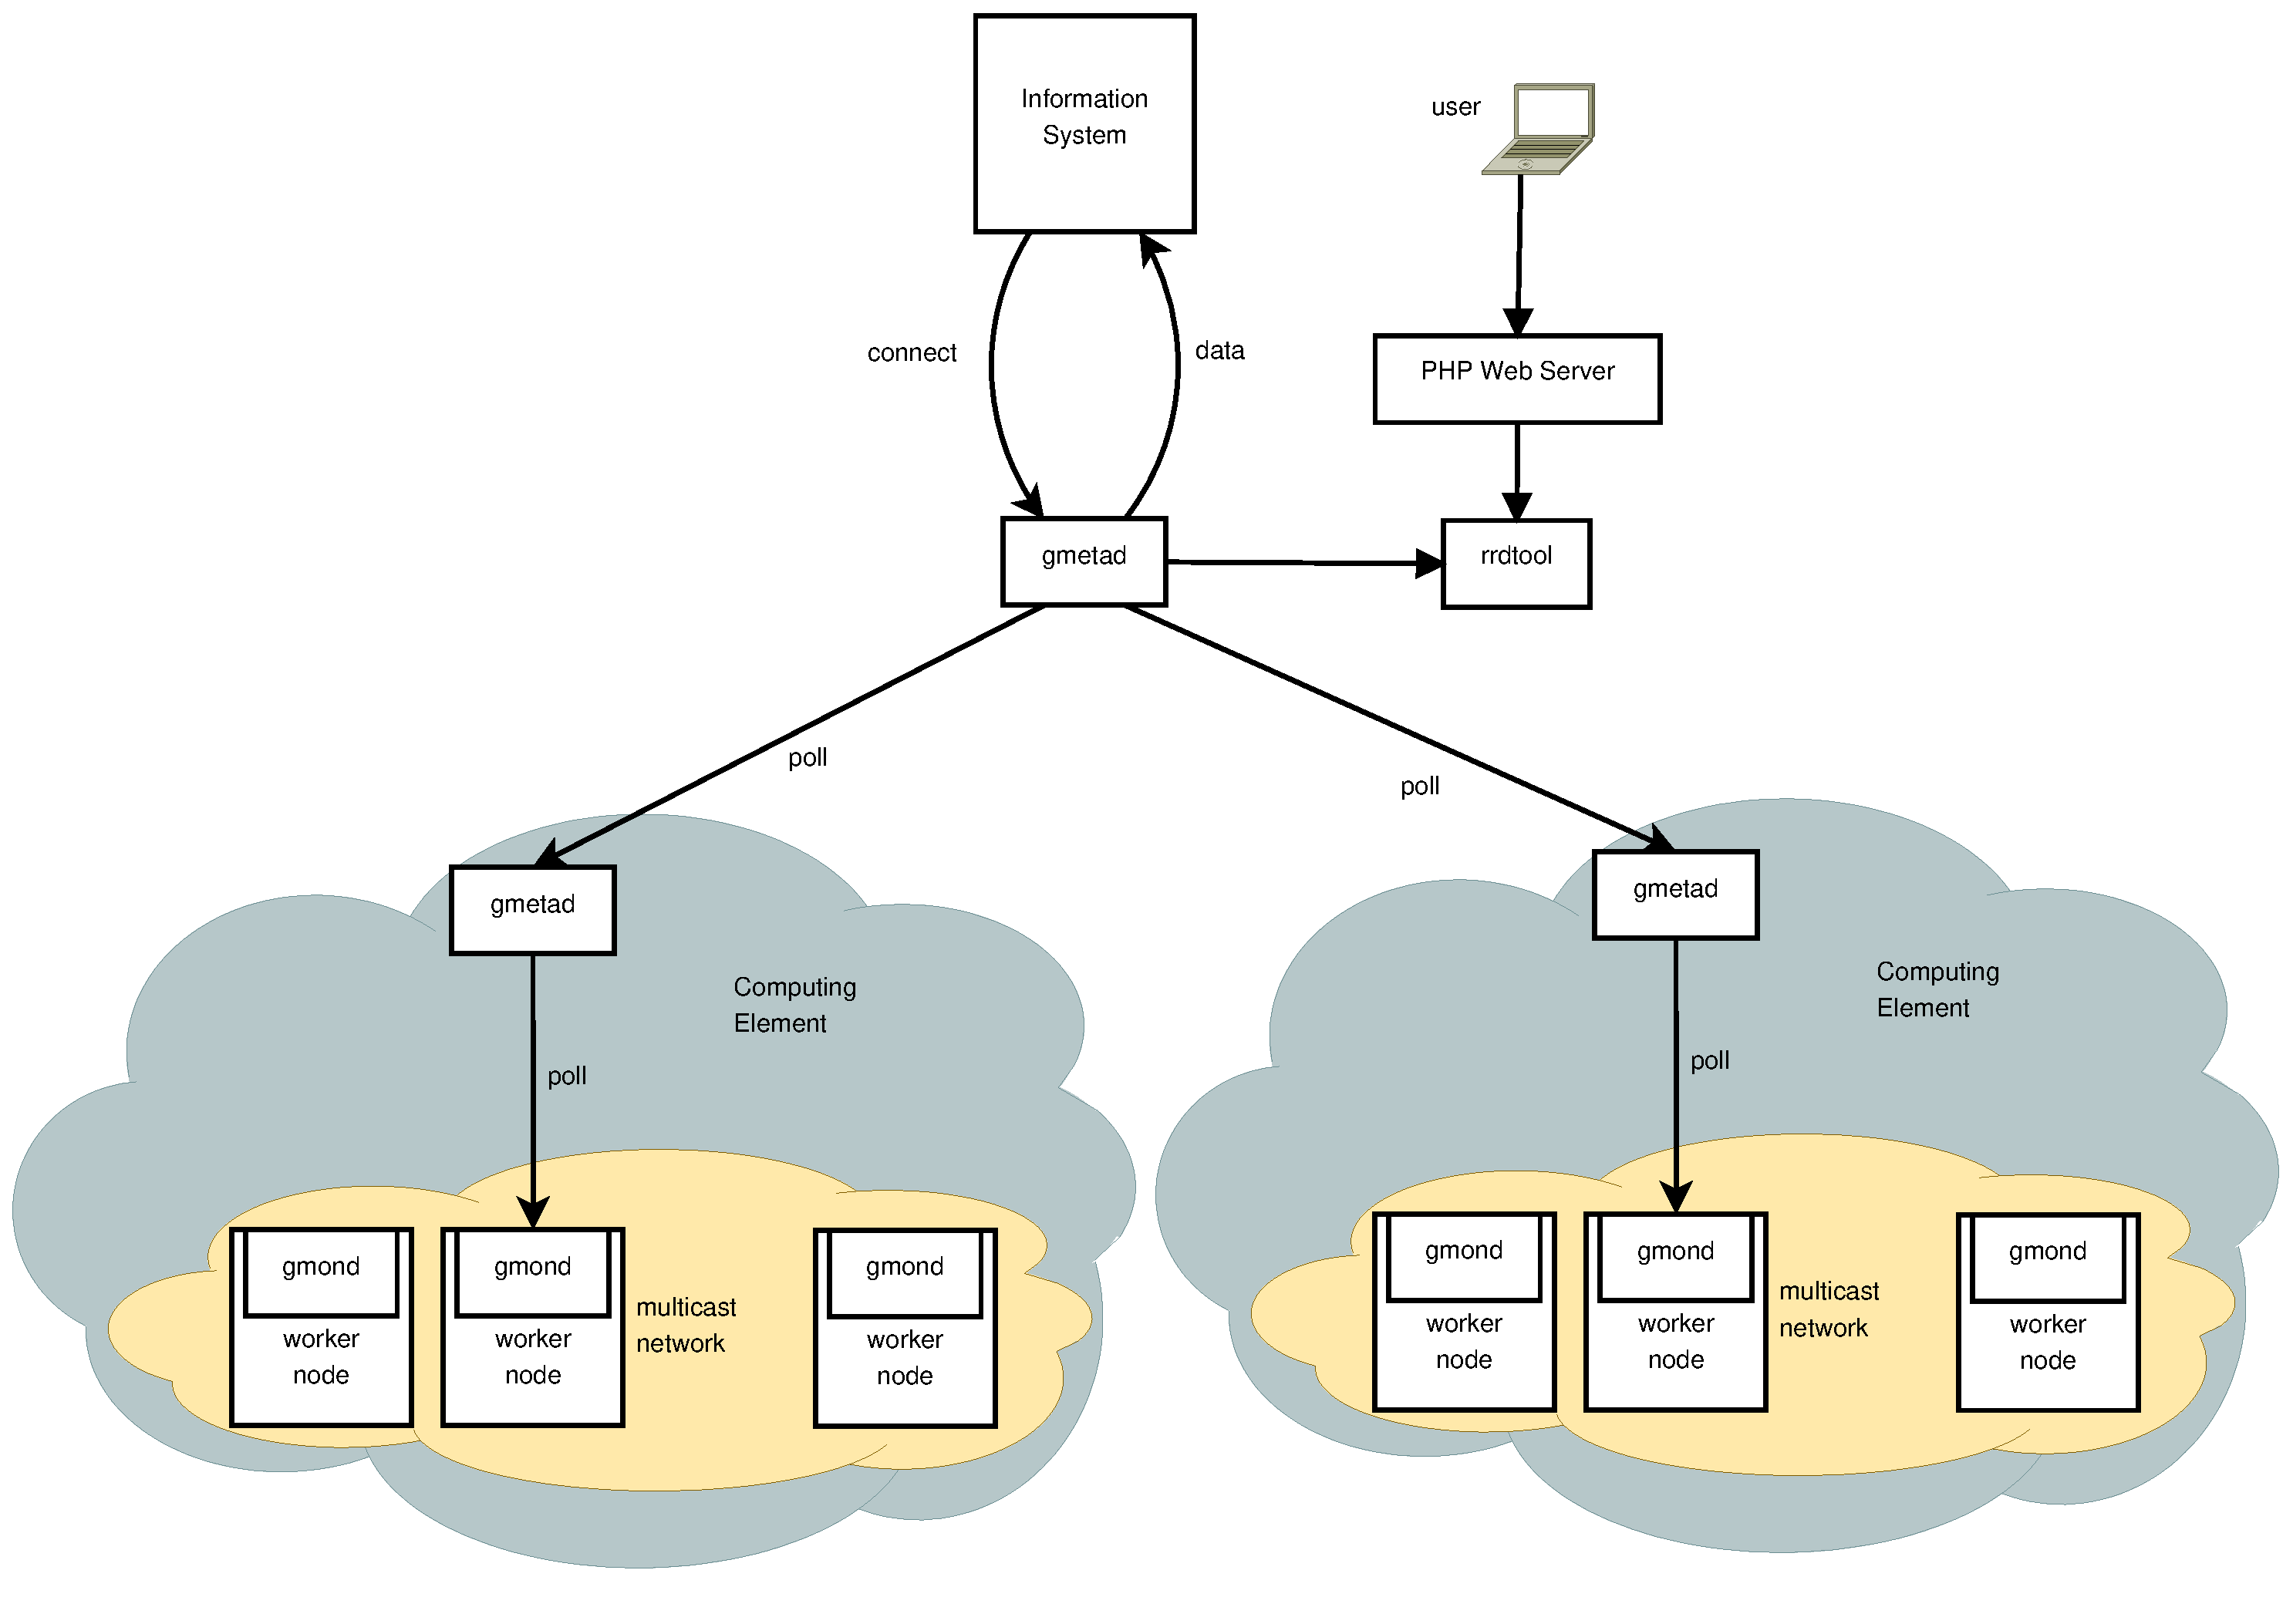
\includegraphics[width=6in]{images/ganglia_data_flow.eps}
\caption{Ganglia Network Communications}
\label{figure:ganglia_network}
\end{figure}


\newpage

\subsection{Nagios}
msg-to-handler msg-nagios-bridge
\newpage

nagios2metric
\newpage

\subsection{Ganglia to Nagios}
check\_ganglia
\begin{figure}[htb]
\centering
 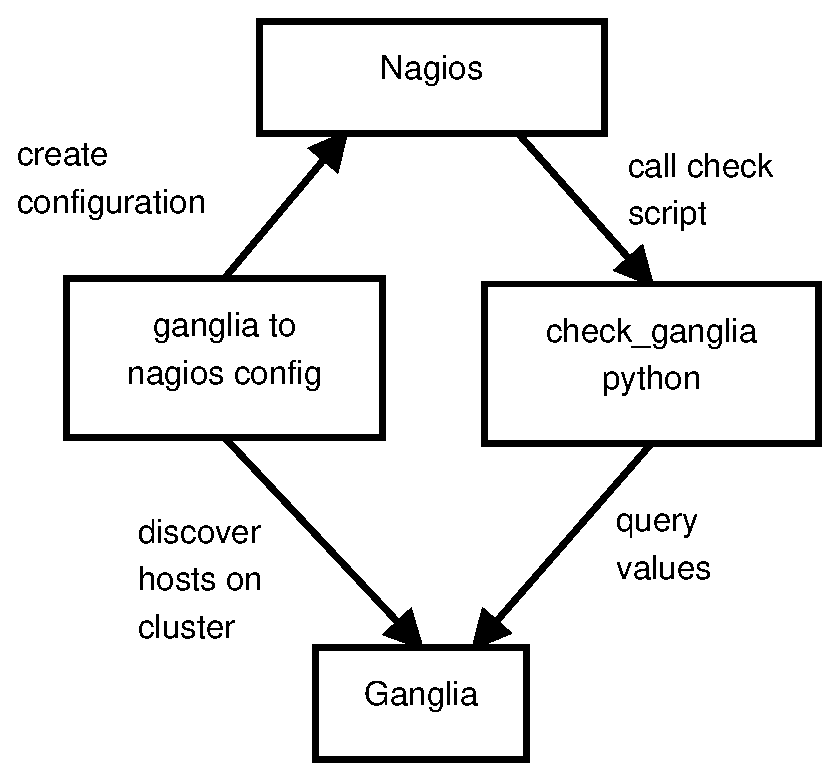
\includegraphics[width=4in]{images/nagios_check_ganglia.eps}
\caption{Nagios configuration and check ganglia values}
\label{figure:nagios_ganglia}
\end{figure}
\newpage

\subsection{pnp4nagios}

Bulk Mode with NPCD
NPCD:
spool directory to process bulk data
create graphs using RRDTOOL

\begin{figure}[htb]
\centering
 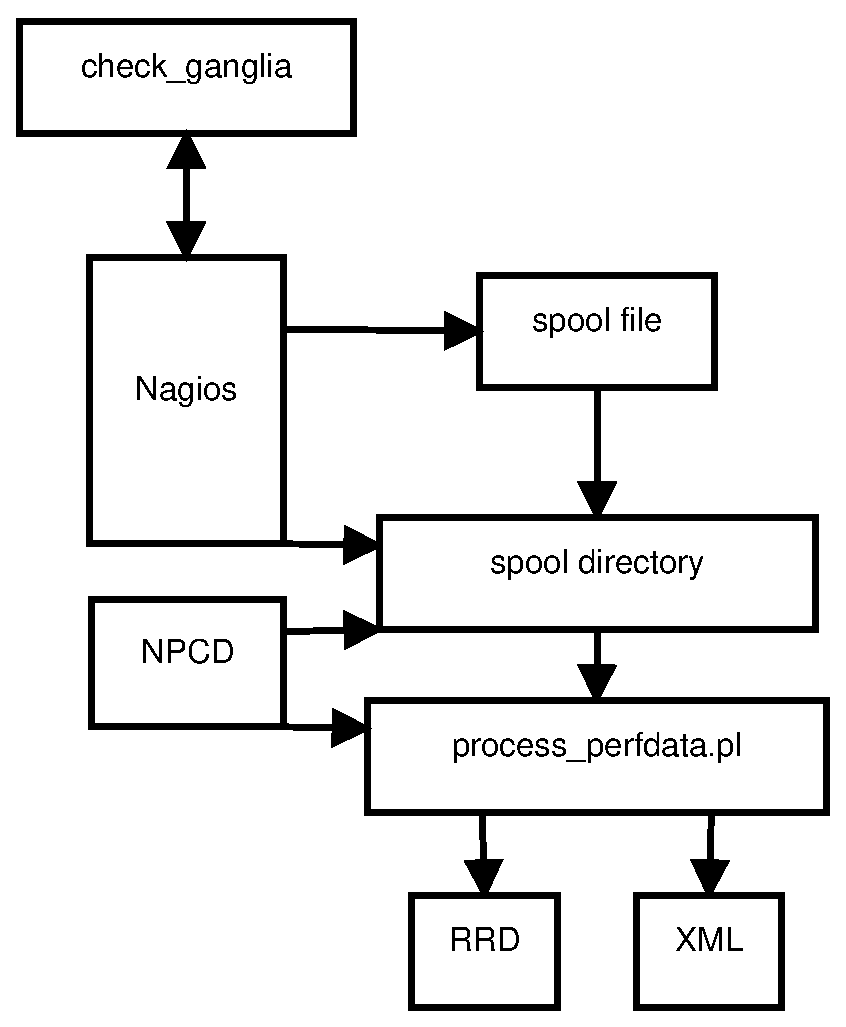
\includegraphics[width=3in]{images/npcd_pnp4nagios.eps}
\caption{PNP 4 Nagios data flow}
\label{figure:pnp4nagios}
\end{figure}
\newpage

\section{Range of cases examined - Metrics}
% here there will be an enumeration of metrics, gmond, etc

Grid performance can be measured using benchmark tools in different levels of the grid architecture, using the micro-benchmarks at the Worker Node level, the Site (CE) level and the Grid VO level. Various benchmarks exist in these levels, using different libraries and algorithms, such as This project focuses on mathematically compute of the performance of a grid based on the metrics that are taken at the Worker Node level.

Different metrics and benchmarks exist, such as the measurement of the performance of CPUs in {\bf MIPS using EPWhetstone} and the evaluation of the performance of a CPU in {\bf FLOP/s and MB/s using BlasBench}. GridBench \cite{gridbench} provides a framework to collect those metrics using its own description language, {\bf GBDL}.

GcpSensor \cite{gcpsensor} introduce a new performance metric called WMFLOPS. It uses PAPI \cite{papi} (Performance API) to access the hardware performance counters. For data distribution it uses MDS information system which provides dynamic metrics for CPU load average, one for 1, for 5 and for 15 minutes load.
\newpage

% TODO ganglia to MDS
\section{Publish to Information System}
\cite{goelagent}

\subsection{LDAP based - MDS/BDII}
To integrate Ganglia with MDS in early versions of Globus, there schema of OpenLDAP should be extended using the Glue-CE definitions from the DataTAG web site (MDS version 2.4). A Ganglia Information Provider was the native ganglia client on python, given by the ganglia development team itshelf.
\begin{enumerate}
  \item Python ganglia client script: \url{http://globus.org/toolkit/docs/2.4/mds/gangliaprovider.html}
  \item Perl gaglia-IP tool: \url{http://www.star.bnl.gov/public/comp/Grid/Monitoring/SimpleGangliaIP.html} and \url{http://www.star.bnl.gov/public/comp/Grid/Monitoring/ganglia\_ip}
\end{enumerate}

\begin{verbatim}
# which glue services does the information base provides?
[root@osweb ~]# ldapsearch -h dgc-grid-44.brunel.ac.uk -p 2170 -x -b "mds-vo-name=uki-lt2-brunel,o=grid" '(&(objectclass=glueservice)(GlueServiceType=*))' GlueServiceType |grep "^GlueServiceType" |sort|uniq

# installation of bdii
-install glite-ui which installs bdii
-ldapsearch bdii
-test perl & python scripts to export mds from gmond
-configure connection to 

[root@osweb ~]# /opt/glite/yaim/bin/yaim -c -s site-info.def -n BDII_site

# configure BDII
site-info.def:
# BDII
CE_HOST="osweb.teipir.gr"
SITE_BDII_HOST="osweb.teipir.gr"
SITE_EMAIL="theofpa@teipir.gr"
SITE_LAT=37.979166
SITE_LONG=23.674719
SITE_DESC="TEI of Piraeus"
SITE_LOC="Athens, Greece"
SITE_WEB="http://oslab.teipir.gr"
SITE_SECURITY_EMAIL=$SITE_EMAIL
SITE_SUPPORT_EMAIL=$SITE_EMAIL
SITE_OTHER_GRID="EGEE"
BDII_REGIONS="oslab.teipir.gr"

\end{verbatim}
\newpage

\begin{table}[ht]
\small\addtolength{\tabcolsep}{-3pt}
\begin{tabular}{ | l | l | r |}
\hline
{\bf Common Name} & {\bf Attribute} & {\bf Objectclass} \\ \hline
Hostname & GlueHostName & GlueHost \\ \hline
Unique ID assigned to the host & GlueHostUniqueID & GlueHost  \\ \hline
Processor Load, 1 Min Average  & GlueHostProcessorLoadLast1Min & GlueHostProcessorLoad \\ \hline
Processor Load, 5 Min Average  & GlueHostProcessorLoadLast5Min & GlueHostProcessorLoad \\ \hline
Processor Load, 15 Min Average  & GlueHostProcessorLoadLast15Min & GlueHostProcessorLoad \\ \hline
SMP Load, 1 Min Average  & GlueHostSMPLoadLast1Min & GlueHostSMPLoad \\ \hline
SMP Load, 5 Min Average  & GlueHostSMPLoadLast5Min & GlueHostSMPLoad \\ \hline
SMP Load, 15 Min Average  & GlueHostSMPLoadLast15Min & GlueHostSMPLoad \\ \hline
Number of CPUs  & GlueHostArchitectureSMPSize & GlueHostArchitecture \\ \hline
Processor Clock Speed (MHz)  & GlueHostProcessorClockSpeed & GlueHostProcessor \\ \hline
Network Interface name  & GlueHostNetworkAdapterName & GlueHostNetworkAdapter \\ \hline
Network Adapter IP address  & GlueHostNetworkAdapterIPAddress & GlueHostNetworkAdapter \\ \hline
The amount of RAM  & GlueHostMainMemoryRAMSize & GlueHostMainMemory \\ \hline
Free RAM (in KBytes)  & GlueHostMainMemoryRAMAvailable & GlueHostMainMemory \\ \hline
\end{tabular}
\caption{GLUE schema for Host Processor Information Provider}
\label{tab:glue}
\end{table}

Perl:
\begin{lstlisting}
$[root@mon ~]# ./ganglia_ip -h mon -p 8649 -o mds
\end{lstlisting}

Python:
\begin{lstlisting}
$[root@mon ~]# /opt/ganglia/bin/ganglia --format=MDS
\end{lstlisting}

\begin{lstlisting}

[root@osweb ~]# cat /opt/glite/etc/gip/provider/glite-info-provider-service-ganglia-wrapper
#!/bin/bash
/opt/bin/ganglia_ip -h 195.251.70.54 -p 8649 -o mds
\end{lstlisting}

\newpage

\subsection{Web Service based - WSRF}
\subsubsection{container}
using WSRF (GT4, information services, information providers)
Ganglia Resource Provider
MDS Index Service
GLUE CE 

OASIS standard

container
\begin{figure}[htb]
\centering
 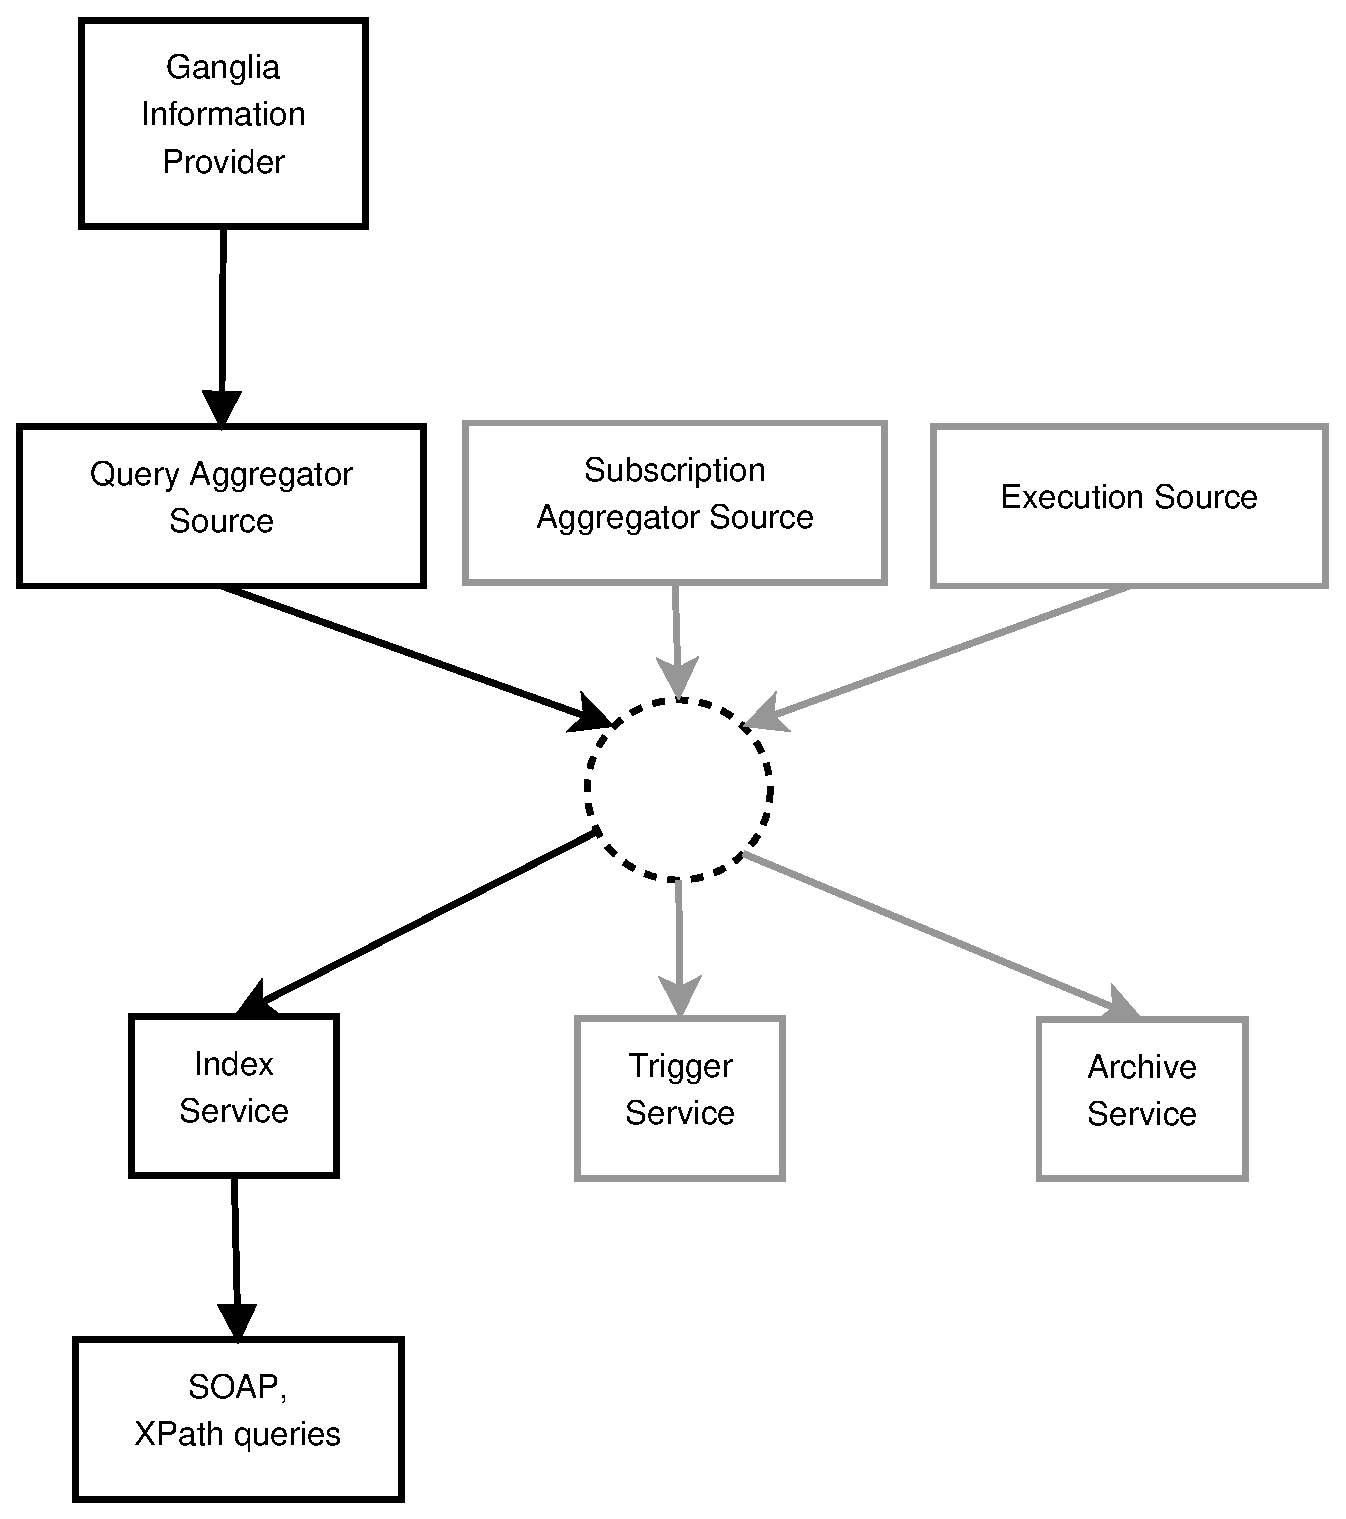
\includegraphics[width=5in]{images/wsrf.eps}
\caption{Web Service Resource Framework}
\label{figure:wsrf}
\end{figure}
\newpage
\subsection{information provider}
wssd

and

rp xml

and

hierarchy.xml maybe in an "aggregation" section

and

deserialization of MDS query in gmond to WSRF
 
\begin{verbatim}
# installation of globus, wsrf, ganglia:
-download binary 4.0.7 and extract to /opt/globus
wget http://www-unix.globus.org/ftppub/gt4/4.0/4.0.7/installers/bin/gt4.0.7-x86_rhas_4-installer.tar.gz
export $JAVA_HOME=/usr/java/default
[root@osweb ~]# export JAVA_HOME=/etc/alternatives/java_sdk
export PATH=$JAVA_HOME/bin:$PATH
./configure
make
make install
-install postgresql, create user & db
-configure globus to connect to postgresql
-create init script for wsrf container
-create ganglia resource provider for wsrf and connect to gmond
-call wsrf to get ganglia metrics

# query WSRF for ganglia data:
[root@osweb ~]# grid-proxy-init -verify -debug
[root@osweb ~]# wsrf-query -s https://osweb.teipir.gr:8443/wsrf/services/DefaultIndexService "//*[local-name()='Host']"
[root@osweb ~]# /opt/globus/bin/wsrf-query -s https://osweb.teipir.gr:8443/wsrf/services/DefaultIndexService "//glue:Host[glue:ProcessorLoad[@glue:Last15Min>20]]"  |grep Load
\end{verbatim}

\newpage
\subsubsection{XPath}

XPath is used to parse an XML document and get a part of it using an address scheme. For XPath, the XML document is a tree consisting of nodes, and its purpose as a language is to get the nodes that are addressed using the XPath query from that document.

Its syntax is compact, non-XML and much like the filesystem addressing, so it facilitates the use of XPath within URIs.

Example queries used in this project are:

The following is used in the PHP code that queries the WebMDS for all nodes of the XML of the WSRF containing nodes with name $Host$:
\begin{verbatim}
//*[local-name()='Host']
\end{verbatim}

Another example is a more complex query that asks the WSRF for all nodes with name $Host$ that contains a sub-node named $ProcessorLoad$ and its $Last15Min$ attribute has value larger than 20:
\begin{verbatim}
//glue:Host[glue:ProcessorLoad[@glue:Last15Min>20]]
\end{verbatim}

Finally the following example may return only the $ProcessorLoad$ node of the $Host$ that has the attribute Name set to $xenia.oslab.teipir.gr$:
\begin{verbatim}
//glue:Host[@glue:Name='xenia.oslab.teipir.gr']/glue:ProcessorLoad
\end{verbatim}

\newpage

\subsubsection{XSLT}
my note: WSRF is GLUE 2.0 schema CE compatible
\begin{verbatim}
file /opt/globus/etc/globus_wsrf_mds_usefulrp/ganglia_to_glue.xslt
\end{verbatim}

\begin{lstlisting}[language=XML,caption=WSRF XSLT for Ganglia Information Provider]
<glue:ProcessorLoad>

<xsl:attribute name="glue:Last1Min">
  <xsl:call-template name="emitProperNumeric">
    <xsl:with-param name="numeric" 
    select="floor(100 * METRIC[@NAME='load_one']/@VAL)"/>
  </xsl:call-template>
</xsl:attribute>

<xsl:attribute name="glue:Last5Min">
  <xsl:call-template name="emitProperNumeric">
    <xsl:with-param name="numeric" 
    select="floor(100 * METRIC[@NAME='load_five']/@VAL)"/>
  </xsl:call-template>
</xsl:attribute>

<xsl:attribute name="glue:Last15Min">
  <xsl:call-template name="emitProperNumeric">
    <xsl:with-param name="numeric" 
    select="floor(100 * METRIC[@NAME='load_fifteen']/@VAL)"/>
  </xsl:call-template>
</xsl:attribute>

</glue:ProcessorLoad>
\end{lstlisting}
\newpage

\subsubsection{WebMDS}
WebMDS is a web interface to query WSRF resource property information. It consists of forms and views of raw XML or organized in tables of results. This user friendly frontend comes as a part of Globus Toolkit version 4 and it can deployed in any application server. Behind this application reside the data that the WSRF aggregation framework provides through the Index Service.

\begin{figure}[htb]
\centering
 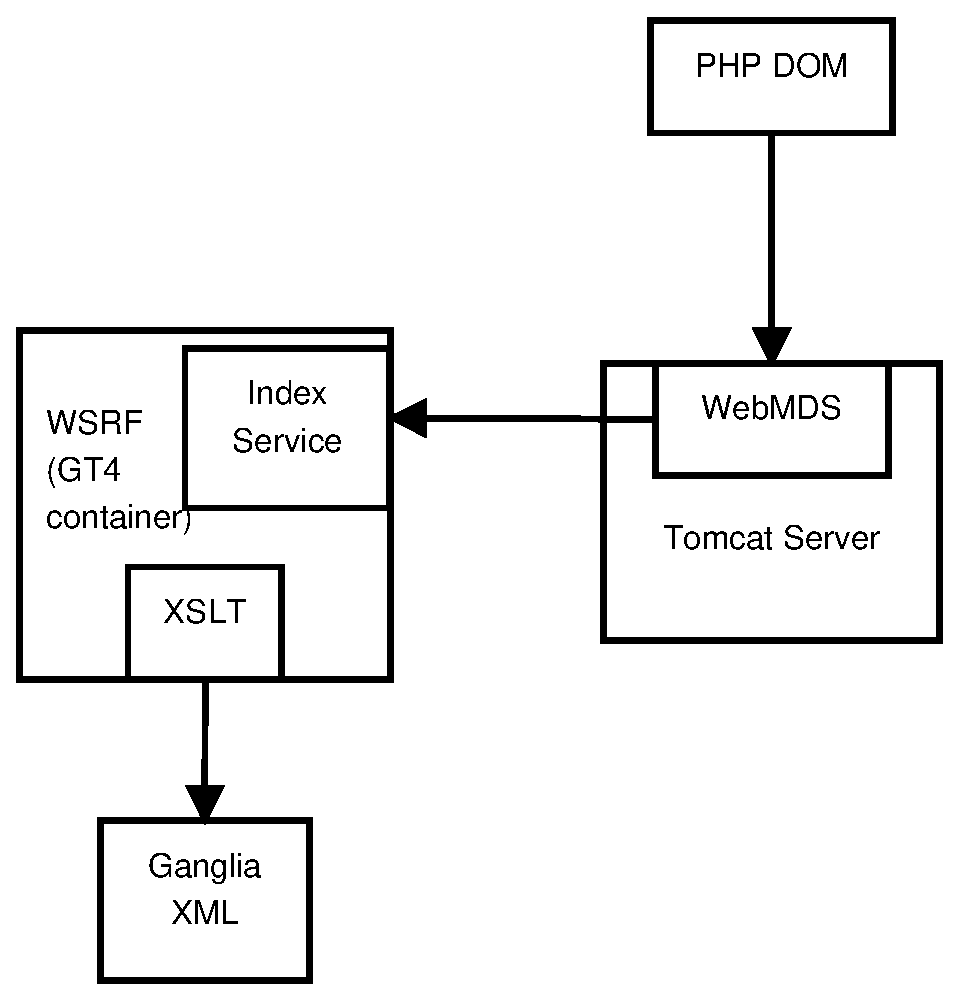
\includegraphics[width=4in]{images/webmds.eps}
\caption{WebMDS application}
\label{figure:webmds}
\end{figure}

For this project an Apache Tomcat server was installed in the box that globus toolkit was running, and the {\bf webmds application} from the GT4 home was deployed. In webmds configuration file, the globa option to allow user specified queries using XPath was enabled.
